\chapter{Recursion}
{ }\hfill\textbf{Level:} Medium\\ \\
\noindent \logo\ programming often uses a technic called recursion. In this chapter, first, we'll explore recursion with some simple examples. Then, we'll go further with the drawing of a fractal curve called the Van Koch snowflake``. First of all:
\begin{center}
\textbf{A procedure is recursive if it calls itself.}
\end{center}
\section{With drawing area.}
\subsection{First example:}
\begin{verbatim}
to ex1
rt 1
ex1
end  
\end{verbatim}
This procedure is recursive because the procedure \texttt{ex1} is called on the last line. While executing, we can see that the turtle turns on itself forever. To break the program, we must click on the STOP button.
\subsection{Second example:}
\noindent Here are three new primitives:
\begin{itemize}
\item \texttt{wait number}\hspace {4cm } \textcolor{red}{ \texttt{wait 60}}\\
Pause the program during the number of 60$^{\textrm{th}}$ seconds. \\
For example, \texttt{wait 120} will pause the program for two seconds.
\item \texttt{penerase}\hspace {4cm } \textcolor{red}{{penerase}}\\
When the turtle moves, it erases all it encounters instead of drawing.
\item \texttt{penpaint}\hspace {4cm } \textcolor{red}{penpaint}\\
Returns to classic mode. The turtle draws lines when it moves.
\end{itemize}
\noindent
\begin{verbatim}
to ex2
fd 200 penerase wait 60
bk 200 penpaint rt 6
ex2
end
\end{verbatim}
Now, we can execute the program. On each second, the same procedure is repeated. We obtain the seconds of a clock!
\section{With the text zone}
\subsection{First example:}
\noindent The primitive \texttt{print, pr} displays text in the text zone. \texttt{print} is waiting for an argument: a list or a word.\\
 Eg: \texttt{pr "hello} \texttt{pr [I write what I want]} (Don't forget the quote " when you want to write only a word.)
\begin{verbatim}
to ex3 :n
print :n
ex3 :n+1
end
\end{verbatim}
Run the command: \texttt{ex3 0} and stop the program with the STOP button.\\
Modify the program to dispay the numbers with an interval of 2.\\
\\
We now want to display all integers greater than 100 which are divisable by 5. We just have to modify the program:
\begin{verbatim}
to ex3 :n
print :n
ex3 :n+5
end
\end{verbatim}
 and then run: \texttt{ex3 100}
\subsection{Breakout test}
\noindent Try the following lines:\\
\texttt{if 2+1=3 [print [it is true]]} \\
\texttt{if 2+1=4 [print [it is true]][print [it is false]]} \\
\texttt{if 2+5=7 [print "true][print "false]}\\
\\
If you doesn't understand yet the syntax of the primitive \texttt{if}, refer to the annex.
\begin{verbatim}
to ex3 :n
if :n=100 [stop]
print :n
ex3 :n+1
end
\end{verbatim}
Then run the command \texttt{ex3 0}\\
Modify the program to display integers between 55 and 350 which are divisable by 11.\\
\section{A fractal example: Van Koch snowflake} \label{vankoch}
\noindent Using recursion, it's very easy to generate in \logo\ some special curves called fractals in mathematics. \\ \\
Here are the first steps to create the Van Koch broken line: 
\begin{center}
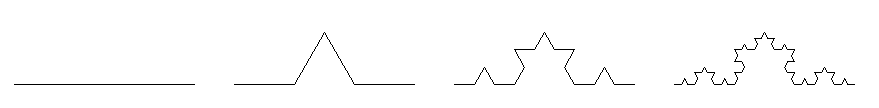
\includegraphics[width=\textwidth]{pics/koch0123.png}
\end{center}
Between two steps:
\begin{enumerate}
 \item each segment is divided into three equal part.
 \item an equilateral triangle is drawn on the middle segment.
 \item finally, this middle segment is erased.
\end{enumerate}
\textbf{What is important:}  Let's have a look at step 2, we  can see that the broken lines contains four identical motifs corresponding to precedent step with a 3 lesser size. Here we have found the recursive structure of the fractal.\\ \\
Let's call $L_{n,\ell}$ the motif of size $\ell$, corresponding to step $n$.\\
To draw this motif:
\begin{enumerate}
 \item We draw $L_{n-1,\ell/3}$
 \item We turn left 60 degrees
 \item We draw $L_{n-1,\ell/3}$
 \item We trun right 120 degrees
 \item We draw $L_{n-1,\ell/3}$
 \item We trun left 60 degrees
 \item We draw  $L_{n-1,\ell/3}$
\end{enumerate}
With \logo, it's very easy to write:
\begin{verbatim}
# :l motif size
# :p step
to line :l :p
if :p=0 [fd :l] [
  line :l/3 :p-1 lt 60 line :l/3 :p-1 rt 120 line :l/3 :p-1 lt 60 line :l/3 :p-1
]
end
\end{verbatim}
If we draw an equilateral triangle with three Van Koch lines, we obtain a beautiful Van Koch snowflake.
\begin{verbatim}
# :l side length
to snowflake :l :p
repeat 3[line :l :p rt 120]
end
\end{verbatim}
Then run: \texttt{snowflake 200 6}
\begin{center}
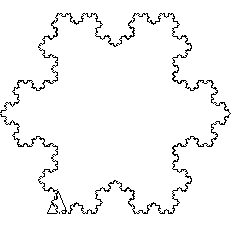
\includegraphics{pics/flocon.png}
\end{center}
\section{Recursion with words}
\noindent Read p.\pageref{liste-prim} to understand how to use the primitives \texttt{word}, \texttt{last}, and \texttt{butlast}.\\ \\
Here is a recursive procedure that inverts the characters of a word.
\begin{verbatim}
to invertword :m
if emptyp :m [output "]  
output word last :m invertword butlast :m
end

print invertword "abcde
edcba
\end{verbatim}
A palindrome is a word, or a phrase that can be read in both sense (Examples: A man, a plan, a canal: Panama ...).
\begin{verbatim}
# test if the word :m is a palindrome
to palindrom :m
if  :m=invertword :m [output true] [output false]
end
\end{verbatim}
Finally, this little kind program, (Thanks Olivier SC):
\begin{verbatim}
to palin :n
if palindrom :n [print :n stop]
print (list :n "PLUS invertword :n "EQUAL sum :n invertword :n)
palin :n + invertword :n 
end

palin 78
78 PLUS 87 EQUAL 165 
165 PLUS 561 EQUAL 726 
726 PLUS 627 EQUAL 1353 
1353 PLUS 3531 EQUAL 4884 
4884 
\end{verbatim} 
\section{Calculate a factorial}
\label{factorielle}
\noindent Factorial of the integer 5 is defined by:
 $$5!=5\times4\times3\times2\times1=120$$
For $n$ positive integer, we can note that: $n!=n\times(n-1)!$.\\
This relation explains the recursive nature of the program:
\begin{verbatim}
to fac :n
if :n=0[output 1][output :n*fac :n-1]
ent

pr fac 5
120
pr fac 6
720
\end{verbatim}  
 \section{$\pi$ Approximation}
\label{approx-pi}approximation
\noindent We can approximate the number $\pi$ using the formula:
$$\pi\approx2^k\sqrt{2-\sqrt{2+\sqrt{2+\ldots\sqrt{2+\sqrt2}}}}$$ with $k$ the number of squareroots. The greater is $k$, the better is the $\pi$ .\\ \\
The formula contains the recursive expression $2+\sqrt{2+\ldots\sqrt{2+\sqrt2}}$, so let's code:
\begin{verbatim}
# k is the number of squareroots
to approxpi :k
write "approximation:\  print (power 2 :k) * squareroot (2- squareroot (calc :k-2))
print "-------------------------
write "pi:\  print pi
end

to calc :p
if :p=0 [output 2][output 2+squareroot calc :p-1]
end

approxpi 10
Approximation: 3.141591421568446 
------------------------- 
Pi: 3.141592653589793 
\end{verbatim}
We found the first 5 digits! If we're looking for more $\pi$ digits, we have to allow a better precision with a higher number of digits while computing. Thus, we're going to use the primitive \texttt{setdigits}.
\begin{verbatim}
setdigits 100
approxpi 100
Approximation: 3.1415926535897932384626433832795028841973393069670160975807684313880468...
------------------------- 
Pi: 3.141592653589793238462643383279502884197169399375105820974944592307816406....
\end{verbatim}
And now, we have 39 digits...